\documentclass[10pt,twocolumn]{article}
\usepackage[spanish,es-nodecimaldot]{babel}
\usepackage[T1]{fontenc}
\usepackage[utf8]{inputenc}
\usepackage{geometry,graphicx,booktabs,hyperref,amsmath}
\geometry{top=1.9cm,bottom=2cm,left=1.7cm,right=1.7cm,columnsep=.65cm}
\title{Entrega 2: textometria y topicos del corpus Duque\\Evidencia exploratoria para analizar framing}
\author{Abel Albuez Sanchez, Kelly Joane Leon Torres,\\Juan Camilo Torres Pena, Jesus David Romero Melo\\\small Maestria en Ingenieria de Sistemas y Computacion, Pontificia Universidad Javeriana}
\date{Octubre de 2026}
\begin{document}
\maketitle
\begin{abstract}
El export contiene 708,768 registros de 6 medios entre 2018-08-07 y 2022-08-06. Hay 707,553 titulos slug y 1,215 ausentes. Se entrenaron K=[3, 5, 7, 10, 15] sobre 706,083 documentos utiles, con 10 pasadas y semilla 42. K=5 obtuvo el mayor c\_v (0.3595) de la grilla. Los resultados son descriptivos de titulos reconstruidos, no estimaciones validadas de sesgo editorial.
\end{abstract}
\section{Objetivo y datos}
El framing no se reduce a sentimiento ni frecuencia de palabras: requiere comprobar seleccion, enfasis y contexto del mismo acontecimiento \cite{entman}. La entrega estudia candidatos lexicos y tematicos del corpus Duque. Los ocho medios corresponden al inventario unificado, no al corte Duque: aqui hay seis, con cinco series principales y Cambio como muestra tardia.
\begin{center}\begin{tabular}{lrr}\toprule Medio & Articulos & Titulos\\\midrule
blu\_radio & 166593 & 165916 \\
cambio & 98 & 98 \\
el\_tiempo & 263145 & 262968 \\
la\_republica & 91801 & 91743 \\
noticias\_caracol & 109384 & 109085 \\
noticias\_rcn & 77747 & 77743 \\
\bottomrule\end{tabular}\end{center}
El corte de fechas es inclusivo 2018-08-07 a 2022-08-06; no filtra automaticamente precision o asignacion presidencial. No hay cuerpos HTML.
\section{Metodo textometrico}
Se normalizan minusculas y tildes en texto y stopwords; se conservan nombres geograficos y actores. Los n-gramas son secuencias despues de filtrar stopwords y nunca atraviesan documentos. El ajuste rango-frecuencia es descriptivo \cite{zipf}; correlacion alta no demuestra ley de potencia. TTR depende del tamano; MSTTR agrega ventanas completas de 50 tokens. Yule K se calcula como $10^4\sum_w f_w(f_w-1)/N^2$ \cite{yule}.
Vocabulario: 98418; tokens: 4737325. Pendiente ajustada: -1.035; R2: 0.969.
\begin{figure*}[t]
\centering
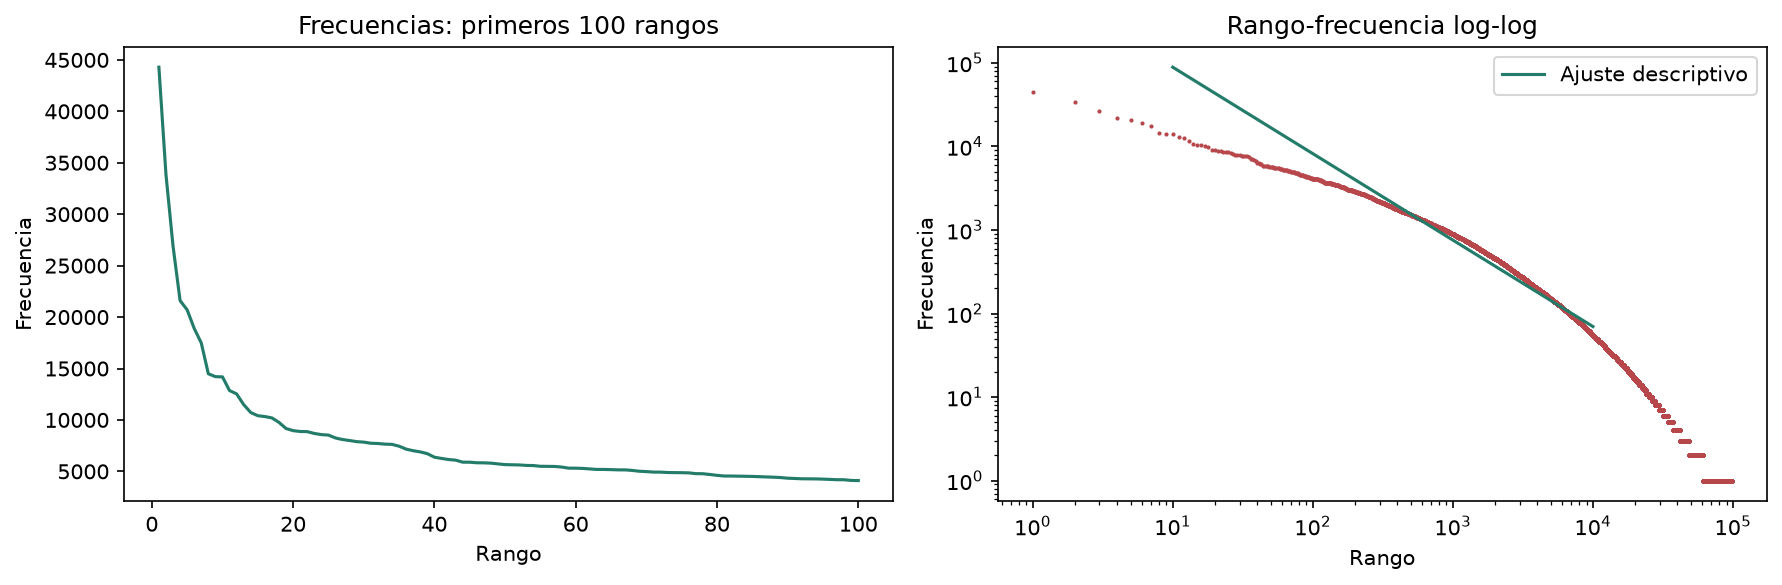
\includegraphics[width=.90\textwidth]{../entrega2/resultados/figuras/zipf_law.png}
\caption{Rango-frecuencia: ajuste descriptivo, no certificacion de ley de potencia.}
\end{figure*}
\begin{figure*}[t]
\centering
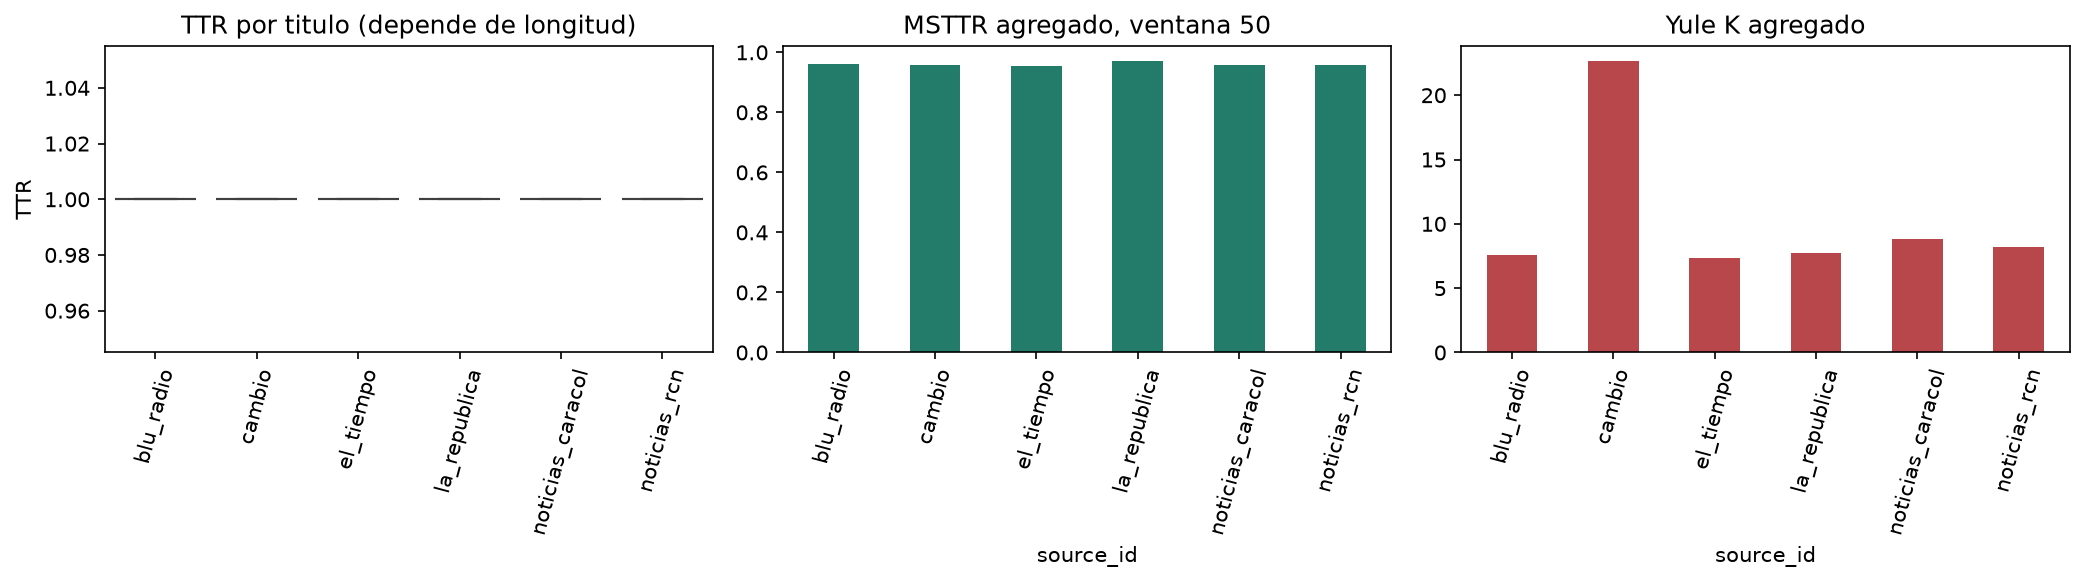
\includegraphics[width=.90\textwidth]{../entrega2/resultados/figuras/lexical_diversity.png}
\caption{Diversidad lexica por medio con indicadores sensibles a longitud.}
\end{figure*}
\begin{figure*}[t]
\centering
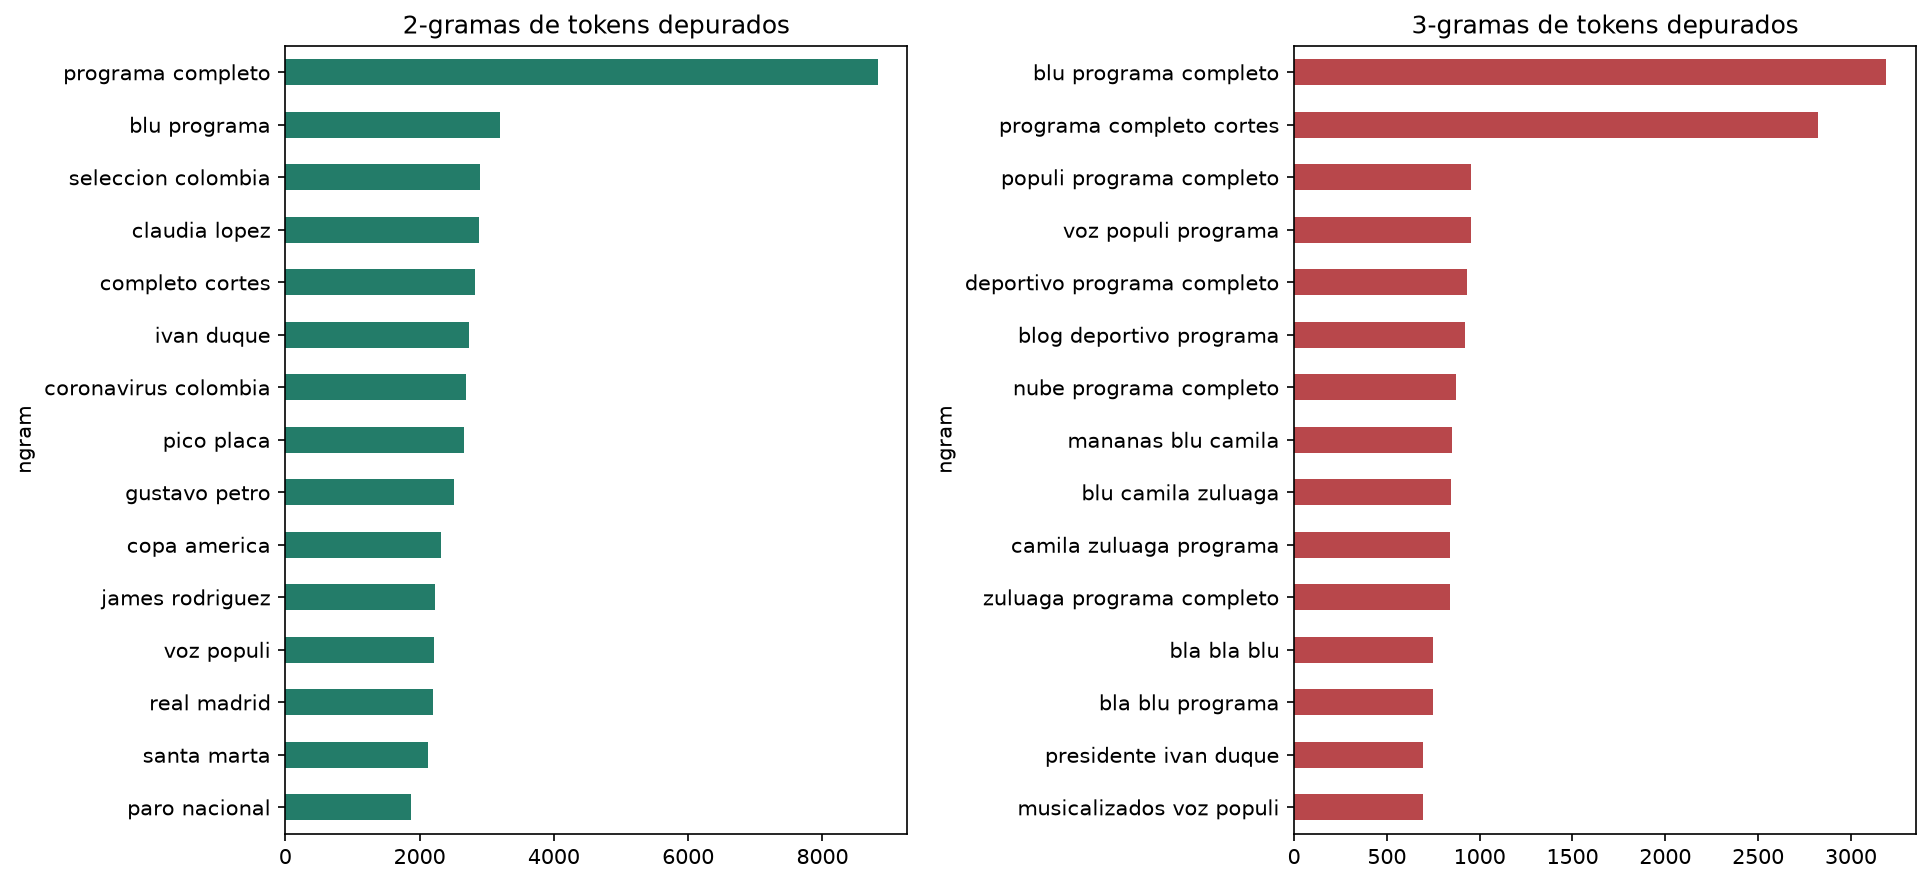
\includegraphics[width=.90\textwidth]{../entrega2/resultados/figuras/ngrams.png}
\caption{N-gramas frecuentes del texto depurado.}
\end{figure*}

\section{Temas y acontecimientos candidatos}
Se buscan Reforma tributaria, Conflicto armado y Corrupcion mediante keywords normalizadas y limites de palabra. Se comparan proporciones sobre titulos disponibles, no conteos como sinonimo de sesgo. Las cohortes pueden solaparse. Se revisan ademas ventanas de reforma/paro 2021, bombardeo/menores 2019 y Centros Poblados 2021. Estos casos y sus ejemplos con URLs son candidatos para comprobacion humana; una coincidencia lexica no certifica el mismo hecho. Los contrastes log-odds son descriptivos y no tienen interpretacion causal.
La Republica tiene 1.08\% de coincidencias tributarias respecto a sus titulos; RCN y Blu registran 1.97\% y 1.97\% en el tema amplio de conflicto. Son proporciones de keywords, no medidas validadas de framing.

\begin{center}{\scriptsize\begin{tabular}{lrrr}\toprule Medio & Tributaria & Conflicto & Corrupcion\\\midrule
blu\_radio & 0.42 & 1.97 & 0.67 \\
cambio & 0.00 & 0.00 & 0.00 \\
el\_tiempo & 0.41 & 1.33 & 0.44 \\
la\_republica & 1.08 & 0.10 & 0.35 \\
noticias\_caracol & 0.32 & 1.66 & 0.51 \\
noticias\_rcn & 0.37 & 1.97 & 0.53 \\
\bottomrule\end{tabular}}\end{center}
Las columnas anteriores son porcentajes de titulos del medio. Cambio (98 titulos) no tiene el mismo alcance temporal; cero coincidencias no prueba ausencia de cobertura.
El bigrama mas frecuente es 'programa completo' (8,822 apariciones). Programacion de radio y emisiones condicionan los resultados; no confundir formato con posicion editorial.
\begin{figure*}[t]
\centering
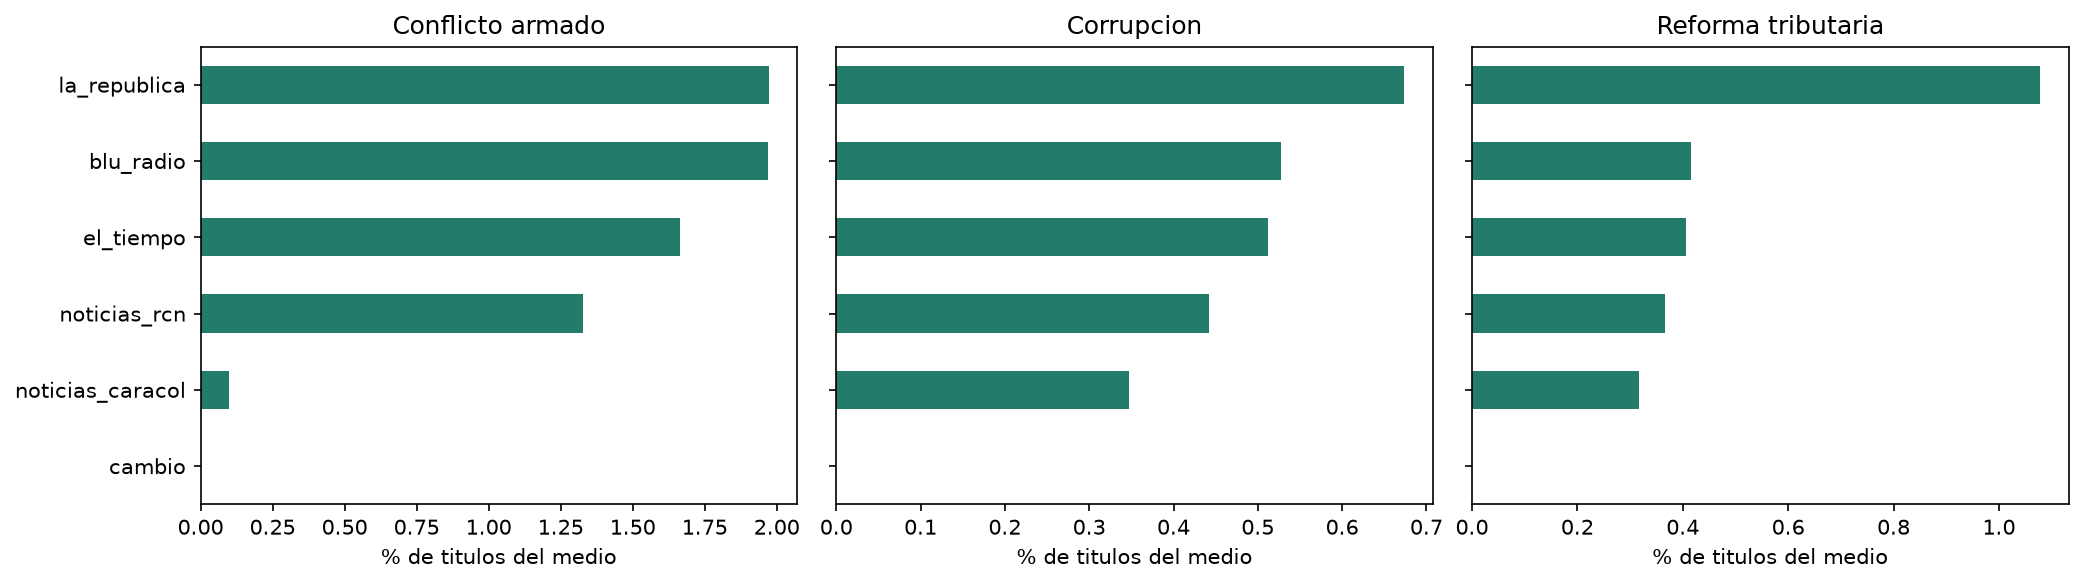
\includegraphics[width=.90\textwidth]{../entrega2/resultados/figuras/eventos_framing.png}
\caption{Cobertura relativa de temas por medio; no es una medicion de framing.}
\end{figure*}

\section{Modelado de topicos}
Se usa LDA \cite{lda} sobre todos los documentos con vocabulario util, sin muestreo. Diccionario: frecuencia documental minima 10, maxima .7 y hasta 10000 terminos. Se entrenan K=3,5,7,10,15, diez pasadas, 50 iteraciones internas y semilla 42. Se elige el mayor $c_v$ de entrenamiento, no un optimo universal. La perplejidad aproximada se transforma desde log-bound en base 2. Documentos sin vocabulario reciben -1, no un topico inventado.
El mejor K de la grilla fue 5 con c\_v=0.3595; documentos utiles: 706083.
\begin{itemize}
\item Topico 0: emision, bogota, martes, jueves, nacional, miercoles, lunes, colombia
\item Topico 1: covid, colombia, dos, bogota, anos, tras, coronavirus, personas
\item Topico 2: colombia, duque, ucrania, unidos, presidente, rusia, gobierno, viernes
\item Topico 3: colombia, asi, video, tras, pico, primera, america, mundial
\item Topico 4: petro, gustavo, luis, caso, diaz, covid, nuevos, fiscalia
\end{itemize}
\begin{figure*}[t]
\centering
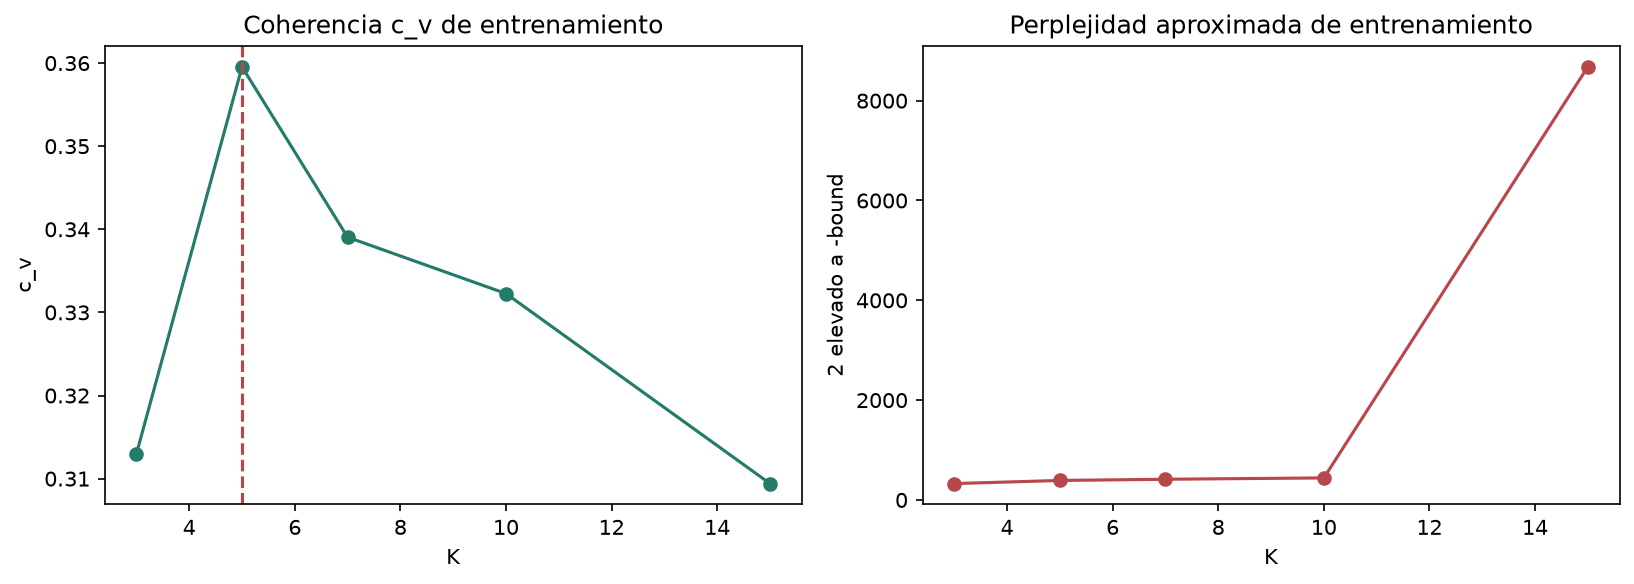
\includegraphics[width=.90\textwidth]{../entrega2/resultados/figuras/lda_optimization.png}
\caption{Comparacion de K: coherencia y perplejidad de entrenamiento.}
\end{figure*}
\begin{figure*}[t]
\centering
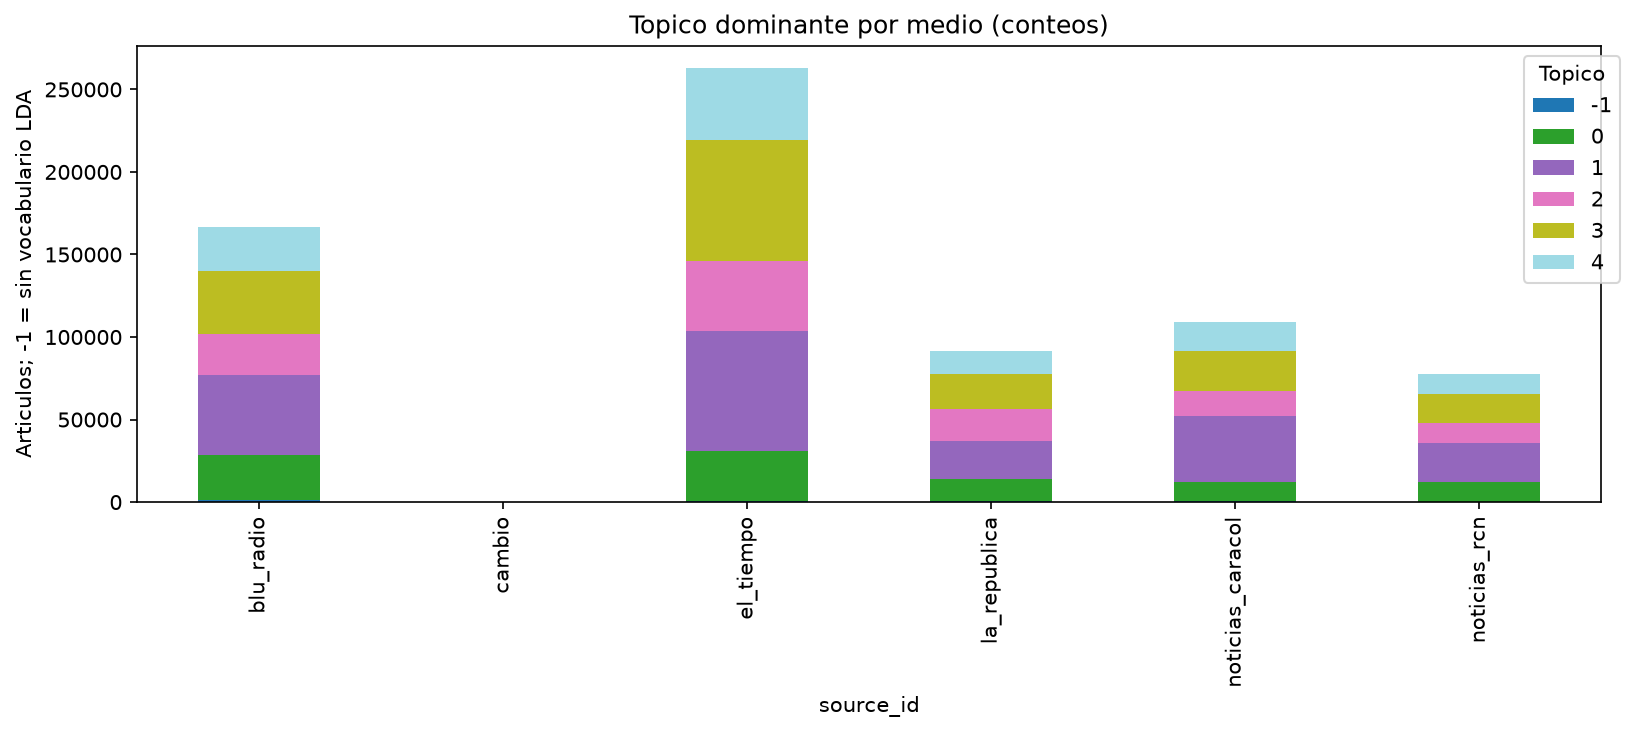
\includegraphics[width=.90\textwidth]{../entrega2/resultados/figuras/topics_by_medium.png}
\caption{Topico dominante: conteos condicionados por el volumen del archivo.}
\end{figure*}
\begin{figure*}[t]
\centering
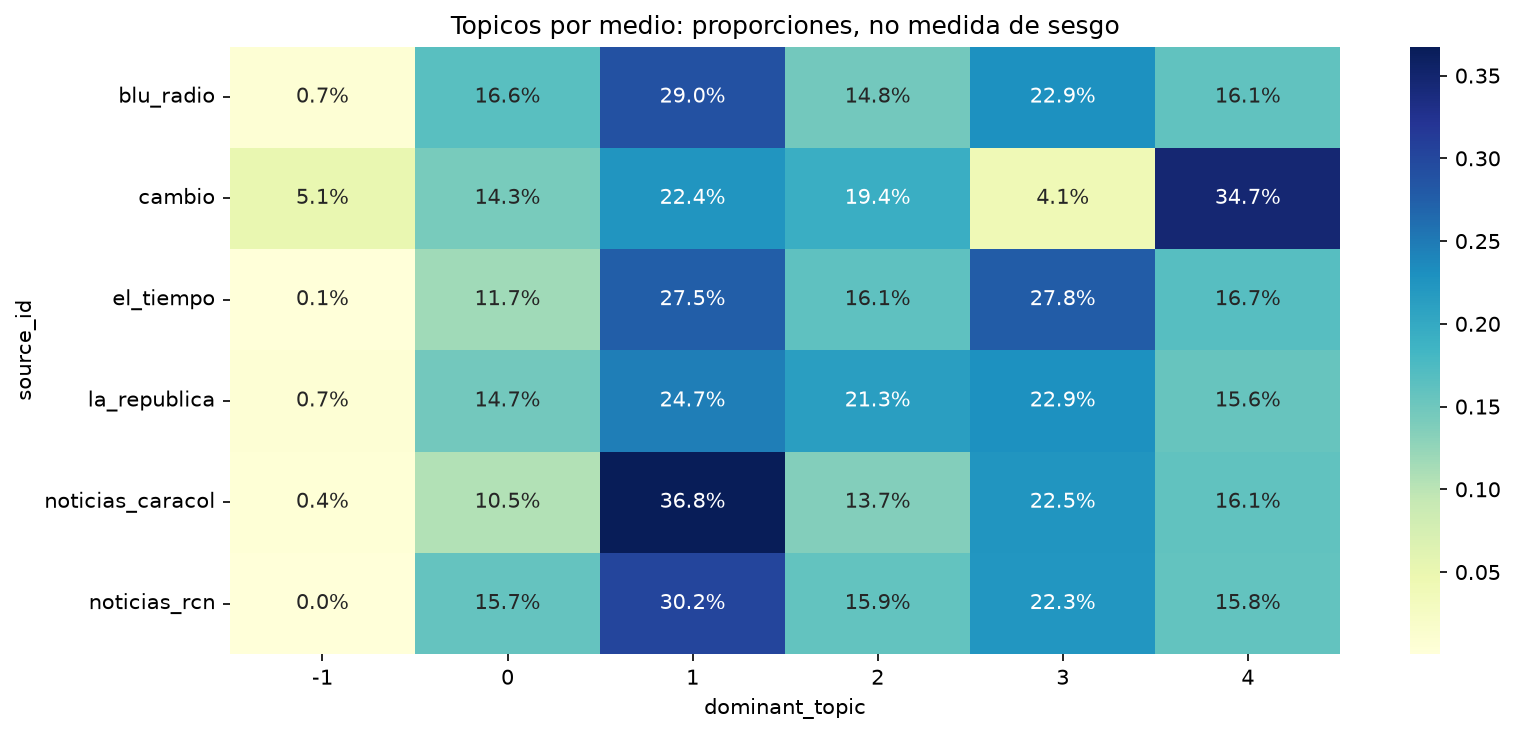
\includegraphics[width=.90\textwidth]{../entrega2/resultados/figuras/topics_heatmap.png}
\caption{Proporciones de topicos por medio.}
\end{figure*}

\section{Limitaciones y conclusiones}
\begin{itemize}
\item Todos los titulos disponibles son proxies slug; no titulares editoriales verificados.
\item No hay cuerpos HTML: no se pueden estudiar citas, actores en contexto o framing textual completo.
\item Cinco medios principales y Cambio con 98 articulos: no ocho medios comparables.
\item Las fechas month y lastmod requieren cautela; un corte por fecha no certifica gobierno.
\item Keywords seleccionan temas/candidatos, no eventos verificados ni omisiones demostradas.
\item LDA/coherencia se evaluan en entrenamiento; el mejor K no es un optimo universal.
\item Programas, emisiones y audio forman parte del archivo; la mezcla de formatos puede dominar las frecuencias.
\end{itemize}
No se concluye que un medio sea mas parcializado. Se obtienen proxies lexicos y de agenda que orientan una submuestra balanceada para recuperar titulares reales/cuerpos, verificar pares de acontecimientos y anotar framing. La comparabilidad requiere controlar fuente de titulo, precision temporal, cobertura de archivo y longitud.
\section{Reproducibilidad}
El notebook integrado carga resultados medidos. Se conservan modelos por K, diccionario, corpus, asignaciones por article\_id, versiones, parametros y SHA-256 del Parquet. No se modifican las bases PostgreSQL ni el export de entrada. Los resultados no sustituyen la validacion manual.
\begin{thebibliography}{9}
\bibitem{entman} R. Entman. Framing: Toward Clarification of a Fractured Paradigm. Journal of Communication, 43(4), 51--58, 1993.
\bibitem{zipf} G. Zipf. Human Behavior and the Principle of Least Effort. Addison-Wesley, 1949.
\bibitem{yule} G. Yule. The Statistical Study of Literary Vocabulary. Cambridge University Press, 1944.
\bibitem{lda} D. Blei, A. Ng y M. Jordan. Latent Dirichlet Allocation. Journal of Machine Learning Research, 3, 993--1022, 2003.
\end{thebibliography}
\end{document}
